\chapter{Available Modules and How to Use Them}
\label{ch:modules}
% ##################################################################################################################

\hfill \textbf{Author:} Andreas Horni, Kai Nagel

\begin{center} 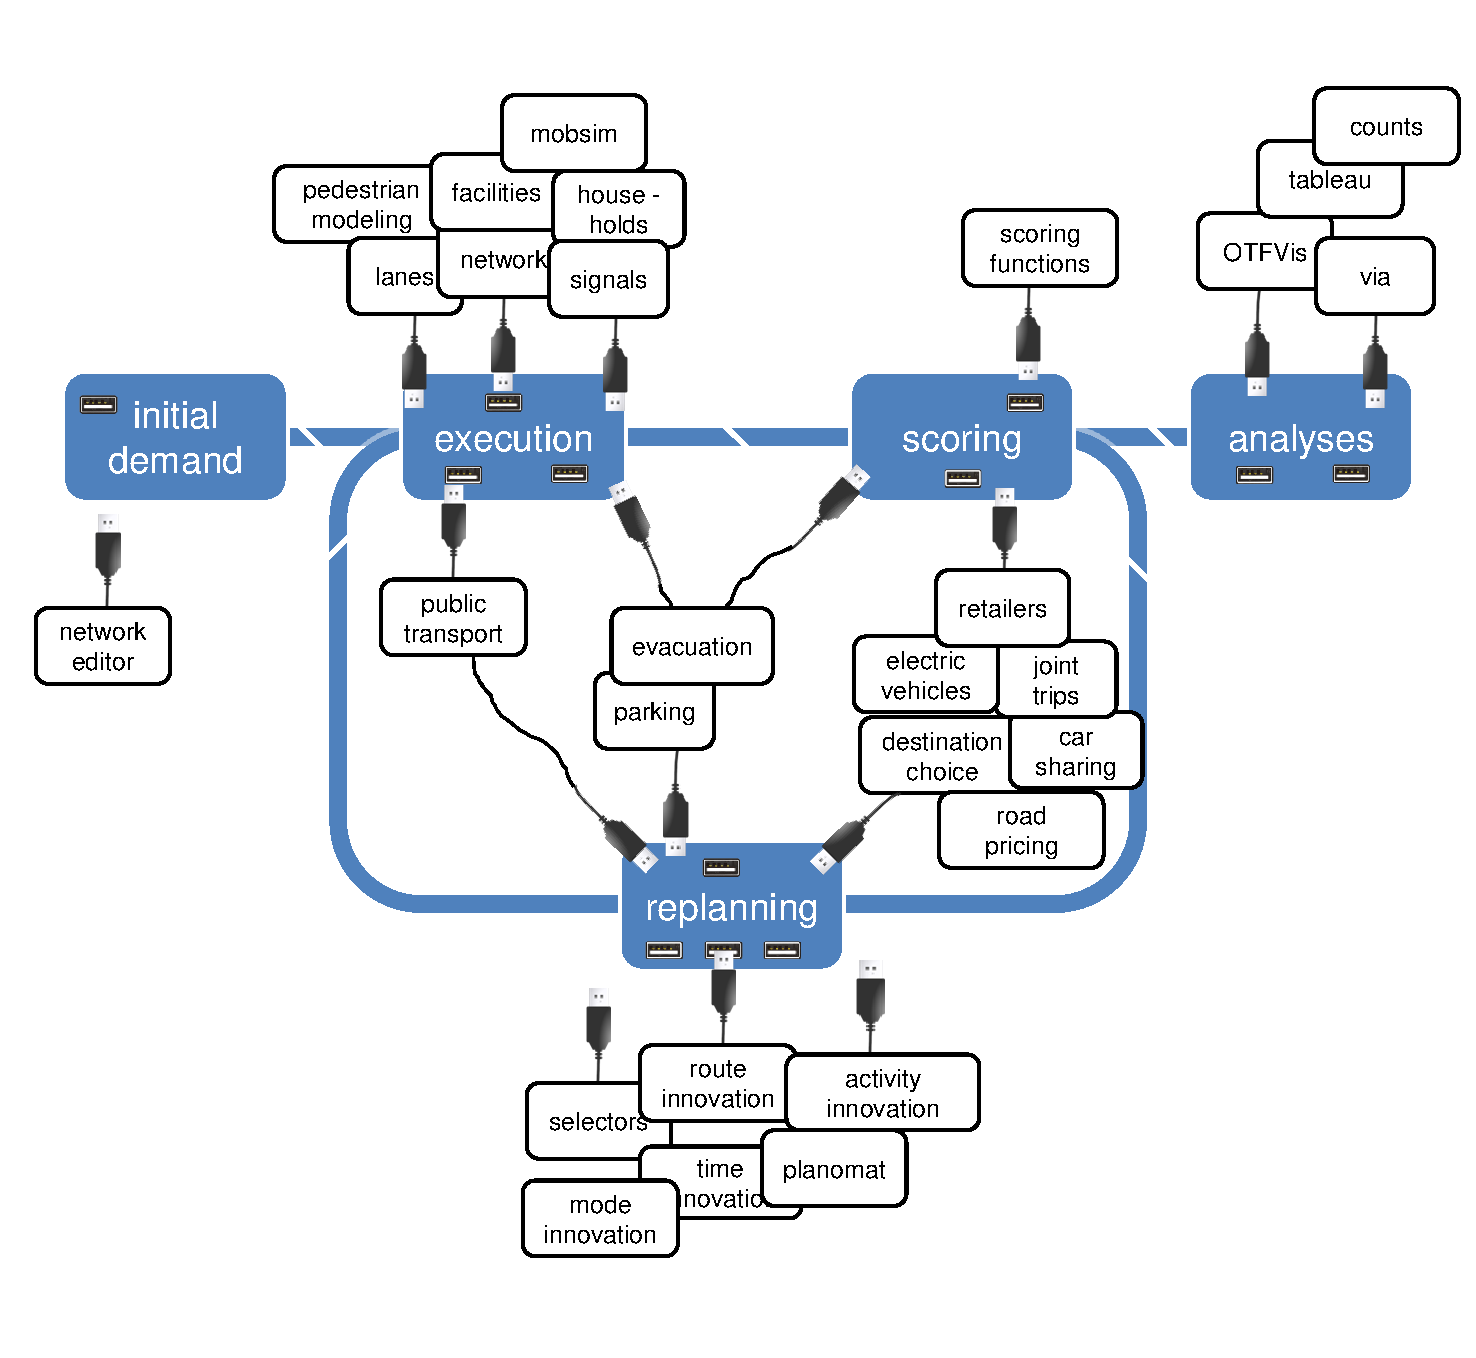
\includegraphics[width=0.5\textwidth, angle=0]{extending/figures/modules.pdf} \end{center}

% ##################################################################################################################
In this chapter you will learn about the possibilities to extend, and customize \gls{matsim} by available functionality. In Chapter~\ref{ch:extensionpoints} you will see how you can hook in your own extensions.

%%\kai{Frage mich im Moment, ob wir diejenigen ``Module'', die man per config aufrufen kann, nicht doch lieber bereits unter ``using'' beschreiben sollten.  Aber vielleicht ist das inzwischen fast egal, und wir sollten lieber Standard-MATSim komplett separat von jeder Art Variation halten.  ???}

% ##################################################################################################################
\section{MATSim Modularity}
\label{sec:matsim-modularity}
\kai{Andreas, haben wir noch eine Chance, diese Ungleichheiten in der Nomenklatur geradezuziehen?  contrib vs extension \url{https://matsim.atlassian.net/browse/MATSIM-323}; PlanStrategy vs StrategyModule; ... }

% ====================================================================================================
\subsection{Levels of Access}
\label{sec:levels-of-access}
\gls{matsim} currently provides four levels of access: using the core only, using core and \glspl{contribution}, writing "scripts in \gls{java}", and finally writing your own \glspl{extension}.

% --------------------------------------------------------------------------------------
\subsubsection{Using the Core Only}
\label{sec:using-core-only}

\kai{würde gerne, hier und im folgenden, url links auf sourceforge gerne vermeiden ... wir haben da keine Kontrolle drüber, ob die sich ändern.  M.E.\ lieber auf so etwas wie matsim.org/downloads verweisen.}

In order to use the core only, one needs to do the following (see Section~\ref{sec:runningmatsim}):
\begin{compactitem}
\item Download a \gls{matsim} release or a nightly build by following the respective links at %% \url{http://sourceforge.net/projects/matsim/files/} or a nightly build \url{http://matsim.org/downloads/nightly} % \kai{url?}.
\url{http://matsim.org/downloads}.
\item Minimally obtain a network file and an initial plans file.  Small versions can be typed by hand; larger versions should be generated automatically by some computational method.
\item Write or edit a config file.
\item Click on the \gls{matsim} jar file\footnote{This works since winter 2014/15 and should be in the 0.7.0 release.} and follow the instructions. 
\end{compactitem}
We think that the \gls{matsim} core is already quite powerful; for example, the synthetic persons already follow full daily plans with a full daily scoring function and in consequence opening times for activity types, departure time choice, and schedule delay can be investigated. Also, schedule-based public transit assignment is contained in the core.

% --------------------------------------------------------------------------------------
\subsubsection{Using One or More Contribs}
\label{sec:using-contribs}

\kai{Das wären jetzt eigentlich extensions; ``contribs'' sind diejenigen extensions, die sich gleichzeitig im matsim repository befinden.  Oder?}

\Glspl{contribution} are in a separate part of the repository, separate from the core.  The documentation is not yet fully organized, information about \glspl{contribution} can be found at \url{http://matsim.org/javadoc} or \url{http://matsim.org/extensions}. There are also release versions and nightly builds, which can be found by following the links at %\url{http://sourceforge.net/projects/matsim/files/} 
%\url{http://matsim.org/files/builds/}. % \kai{check} \ah{gibt es beides am gleichen Ort wie MATSim} \kai{url?}.
\url{http://matsim.org/downloads}.

In general, \glspl{contribution} should provide main methods with which they can be used.  We might eventually provide clickable jar files here as well, but for the time being the extensions need to be bundled with core \gls{matsim} (and potentially other \glspl{contribution}). As shown at \url{http://www.matsim.org/docs/extensions} the syntax roughly is
\begin{lstlisting}
java -Xmx2000m -cp MATSim.jar:contrib/contrib.jar org.matsim.contrib.run.Main config.xml  
\end{lstlisting}
%% \kai{Maybe better point to electronic docu?} \ah{command ist unter url oben gegeben}
where
\begin{compactitem}
\item \lstinline$-Xmx2000m$ increases the \gls{java} heap space so that most \gls{matsim} runs fit in
\item \lstinline$MATSim.jar$ needs to be replaced by a relative or absolute path to the \gls{matsim} jar to be used
\item \lstinline$contrib/contrib.jar$ needs to be replaced by a relative or absolute path to the \gls{contribution} jar to be used
\item \lstinline$org.matsim.contrib.run.Main$ needs to be replaced by full \gls{java} class name containing the desired main method (given by the \gls{contribution} documentation)
\item \lstinline$config.xml$ needs to be replaced by a relative or absolute path to a config file, which may contain additional sections specifically for the \gls{contribution}
\end{compactitem}

It is possible to combine several \glspl{contribution} in this way, provided someone has made available a corresponding main method.  This can in principle be done relatively quickly, so persons who want to run studies with combinations of existing \glspl{contribution} but without programming skills can ask someone with those skills and with access to the repository to help.

% --------------------------------------------------------------------------------------
\subsubsection{Writing "Scripts in Java"}
\label{sec:writing-scripts-java}
The \glspl{contribution} are written in a style that they can be plugged into core \gls{matsim} via extension points (see Chapter~\ref{ch:extensionpoints}). If a specific combination or configuration of modules is not (yet) available, one can write it for oneself. The syntax roughly is
\begin{lstlisting}
... main( ... ) {
    // construct the config object:
    Config config = ConfigUtils.xxx(...) ;
    config.xxx().setYyy(...) ;
    ...

    // load and adapt the scenario object:
    Scenario scenario = ScenarioUtils.loadScenario( config ) ;
    scenario.getXxx().doYyy(...) ; // (*)
    ...

    // load and adapt the controler object:
    Controler controler = new Controler( scenario ) ;
    controler.doZzz(...) ; // (**)
    ...

    // run the iterations:
    controler.run() ;
}
\end{lstlisting}
The extension points, especially at \lstinline{(*)} and \lstinline{(**)}, are described in more detail in Chapter~\ref{ch:extensionpoints}.

% --------------------------------------------------------------------------------------
\subsubsection{Writing Your Own Extensions}
\label{sec:writing-your-own-extensions}
If the existing \glspl{contribution} are not sufficient to plug your own study together, the next option is to write your own \gls{extension}.  Again, this should preferably use the extension points described in Chapter~\ref{ch:extensionpoints}, since this is the only way in which an \gls{extension} may later become a \gls{contribution}.  \kai{here is a difference between an extension and a contrib :--)}

%% \paragraph{If none of this is enough}
%% Clearly, it is always possible to download some version of \gls{matsim}, remove all the \lstinline{final} 

% ====================================================================================================
\subsection{The Ideas Behind this Setup}
The setup as described above came out of the observation that an ever growing monolithic \gls{matsim} would eventually overwhelm the core team. Therefore, a set-up was searched where the core team could concentrate on central infrastructure, while specific functionality such as road pricing, multi-modal simulations, signals, additional choice dimensions, or analysis modules could be written and contributed by other people. Clearly, a plug-in architecture had to be the solution, but it took (and still takes) time and effort to make the extension points sufficiently capable and sufficiently robust.  

At the same time, \gls{matsim} is a research platform, and a trait of research is that it investigates innovative questions, which often means that the questions were not foreseen by the designs of the code.  Quite often, scripting languages are the solution to such problems; for example, QGIS or VISUM allows python \cite{...} for plug-ins; EMME allows ???; SUMO allows ??? \kai{traci}.  Scala \cite{...} was discussed for \gls{matsim}, but in the end it was decided to just use Java itself as the scripting language. This has the advantage that persons who are in between core development and \gls{matsim} application do not need to learn two languages, and in addition the TUB team can continue to teach \gls{java} both as an entry point to \gls{matsim} and as a general professional skill.

% ====================================================================================================
\subsection{MATSim Modules}
According to the Merriam-Webster (\url{http://www.merriam-webster.com}), a module is
%
"one of a set of parts that can be connected or combined to build or complete something" 
%
or more specifically
%
"a part of a computer or computer program that does a particular job". 
%
That is, "module" is not a very specific term, and in consequence modules exist in \gls{matsim} at many levels. Metaphorically speaking, the term module can thus be seen as the greatest common divisor (gcd) of different functionality as listed below.
%% , so to say, a module is the \lstinline|AbstractClass| of \gls{matsim} functionality. 
%
% Eine abstrakte Klasse im Java-Sinne ist ein nicht einfaches Software design Konzept; das würde ich hier nur ungern nennen. kai, jan'15
As \gls{matsim} is 
highly modular, it nevertheless makes sense to think of functionality wrapped by a module. In the following are some important examples.

%% The basic concept to extend MATSim is the usage of modules. But, please be aware that when it comes to configuring MATSim the term ``module'' is very extensively used such that a clear definition of what is a module and what is not is not available to date. This consequence of organic grows be corrected on the long run, for now, we try to just sort out the different meanings of the word module

%% \kai{Ich bilde mir ein, dass wir das im Kopf schon etwas klarer haben, als es historisch noch aussieht, und würde gerne versuchen, das hier zu kommunizieren.  Ich habe in der Einleitung zu Kap.~\ref{ch:extensionpoints} etwas geschrieben, was man vielleicht inhaltlich auch hier verwenden kann ...}

%% Following different components are called modules.

%% \paragraph{Components in \lstinline|org.matsim|:} % --------------
% ...........................................................................
\paragraph{Config Modules:} The config \gls{xml} file uses a syntax of the type
\begin{xml}
<module name="aModule">
    <param name="aParameterForAModule0" value="someValueX" />
    <param name="aParameterForAModule1" value="someValueY" />
</module>
\end{xml}
The config modules loosely correspond to components providing distinct functionality. 

%% residing in the \lstinline|org.matsim| package.  

%% Habe das mal auskommentiert.  Ist erstens eine Null-Aussage (alles ist unterhalb von org.matsim, auch die contribs), und zweitens ist es wenigstens im Java-Sinne keine package (oder genauer: Gerade in dieser package ist nichts drin). kai, dec'14

{\footnotesize

\kai{Andreas, habe obige Argumentation mal umgedreht.  Du bist von der code Struktur zum config file gegangen.  Ich gehe jetzt vom config file aus, und erwähne den code nur beiläufig.  Grund: Die beiden hängen tatsächlich nicht besonders stark zusammen.  Insbesondere passen wir die config, wg. Rückwärts-Kompatibilität, praktisch nie an strukturelle Änderungen im Code an.  (Abgesehen davon ist die config Struktur gar nicht so schlecht; problematisch finde ich teilweise eher die Benennungen.  Ein Favorit: ``planCalcScore'' (ohne s hinter plan) vs ''plansCalcRoute'' (mit s hinter plan). Oder?)}

}
% ...........................................................................
\paragraph{Replanning Modules:} Package \lstinline|org.matsim.core.replanning.modules| provides replanning functionality that can also be plugged into \gls{matsim}. 

%% A slightly different meaning of modules, which is only relevant for the MATSim developer and API-user, is as follows. In the package package \lstinline|org.matsim.core.replanning.modules| replanning functionality is provided in classes that are derived from \lstinline|AbstractMultithreadedModule|.

\kai{Dies ist mein zweiter Favorit.  ``(strategy)module'' in der config, aber ``PlanStrategy'' im code, die dann wieder ``PlanStrategyModule''s akzeptiert.  Schaffen wir es, dies aus Anlass des Buches zu ändern?  Siehe \url{https://matsim.atlassian.net/browse/MATSIM-306}.  Bitte äußere Dich dort (kann ja kurz sein).}
\ah{Hab mal gevoted. Viel Zusätzliches zu sagen gibt es ja nicht ;)}

\kai{Lasse das bis zur Klärung dieser Frage mal offen.}

% ...........................................................................
\paragraph{Contributions:} \Glspl{contribution} are modules residing in the \lstinline|org.matsim.contrib| package.

\kai{Von mir aus können wir das durchgängig ``contribs'' oder ``contributions'' oder ``extensions'' nennen.  Leider hat Marcel für die package einen anderen Namen (contrib) gewählt als für die Doku (extensions).  Aber ``module'' muss nicht sein.}
%
\ah{Könnten wir sie trotzdem als Modul bezeichnen (einfach mit weniger negativem Unterton)? Die Story wird sonst sehr unübersichtlich (auch Kapitel "`Your Own Modules/Extensions...). Die anderen Probleme mit dem inflationären Gebrauch des Begriff bleiben ja.}
%
\kai{Verstehe das Argument.  Andererseits wird es auch nicht einfacher, wenn wir die Sprache nicht konsistent halten.  Hm.}

\ah{Aus meiner Sicht ist "Modul" einfach der ggT oder die AbstractClass der verschiedenen Arten von ... Funktionalitäten (und somit eigentlich nutzlos?). Jedenfalls würde ich sie hier doch als Module bezeichnen, da sie sonst auch aus diesem Kapitel raus müssten.}

\ah{Habe das oben mal (noch etwas blumig) angepasst.}

% ...........................................................................
\paragraph{External Functionality:} % --------------
Also external components plugged in and replacing a \gls{matsim} module, such as a \gls{mobsim}, can be interpreted as modules.

\gls{matsim} provides the possibility that the parameters of arbitrary external modules are added to the configuration file as detailed above. In the respective module, the parameters can be accessed in two ways. The suggested way is extended the \lstinline|Config| object to include an external config group as follows.
%
\begin{lstlisting}
MyExternalConfigGroup myConfig = ConfigUtils.addOrGetModule(controler.getConfig(), MyExternalConfigGroup.GROUP_NAME, MyExternalConfigGroup.class);
\end{lstlisting}
%
Parameters are then available by the getter methods of \lstinline|MyExternalConfigGroup|. A second way, is using the following command of the \lstinline|Config| class.
\begin{lstlisting}
public final String findParam(final String moduleName, final String paramName)| 
\end{lstlisting}
Note, that here, the user's input is not checked while reading in the \gls{configfile} but much later, possibly in the external module.

\kai{MZ, wollen wir dieses findParam eigentlich noch "advertisen"?  Bisher ist es immer darauf hinausgelaufen, dass ich das irgendwann durch eine "typisierte" config group ersetzt habe.  M.E.\ könnte man zukünftig auch gleich mit einer typisierten config group anfangen.  Oder?}
\ah{Hab mal beides hingeschrieben. Michael: Ist eines von beidem immerhin empfohlen? ;)}

% ...........................................................................
\paragraph{Standalone Tools:} % --------------
Also the standalone tools referencing \gls{matsim} as a library, such as the network editor, or the visualizer via, can be seen as modules.
%are termed modules in current practice.


% ===================================================================================
%\subsection{Current Problems With Modules}
%
%\kai{Habe diesen ganzen Abschnitt mal probehalber auskommentiert.  Module können auf vielen Ebenen auftreten, dass sie das tun, ist kein Fehler.  Manche der Aspekte können wir immer noch in den spezifischen Kapiteln beschreiben (es gibt tatsächlich einen Grund, warum es die ganzen unterschiedlichen mode innovation modules gibt); manche können wir vielleicht noch vor Fertigstellung des Buches im Code aufräumen.}

%% The majority of the replanning modules have their own section in the configuration file, but some do not, such as the \lstinline|TripsToLegsModule|. 
%% \kai{Aber warum ist das ein Problem?  Die sind halt nicht weiter konfigurierbar.}
%% %
%% In that package---called modules---there are furthermore, the factories for the plan selectors. For the selectors and their factories, it is unclear if they are modules.
%% \kai{factories sind keine modules, sondern extension points, um module zu erzeugen und in den code zu stöpseln.  Selectors selber sind PlanStrategies und insofern modulare Bestandteile.}

%% To make things worse, there are cases where module names in the configuration file are not (yet) consistent with the naming in the code. Examples are ``\lstinline|strategy|'' in the configuration file and ``\lstinline|StrategyManager|'' in the code, or ``strategy module'' in the config file and ``\lstinline|PlanStrategy|'' in the code \ah{Nochmals nachsehen!}. Furthermore, modules are atomic. There is, for example, a module called ``\lstinline|ChangeSingleLegMod|'', a module ``\lstinline|ChangeLegMode|'' and a module ``\lstinline|SubtourModeChoic|'' instead of one single module called ``\lstinline|ModeChoice|''. This, on the one hand, has historical reasons; the three modules were developed temporally separated. On the other hand, the parameter set for a module is only minimal and unambiguous if provided for atomic modules as different parameters are required for the three modules.

%\ah{Habs noch ganz auskommentiert.}

% ##################################################################################################################
\section{An Overview of Existing Modules}
Figure~\ref{fig:matsimmodules} shows where in the \gls{matsim} loop, common \gls{matsim} modules are plugged in. Some modules are already presented in Chapter~\ref{ch:configuring}, while here, it is shown how functionality can be extended beyond using the \gls{configfile}, population and a network only. The technical details for module usage, in particular the parameter sets are described in \citep[][]{MATSim_Userguide_2015} and in the javadoc.

For the presentation of the available functionality, we chose to not use a single section per module but to group them according to common transport planning categories, in the example above this would be "mode choice" instead of the atomic categories, where we use terms "functionality" for the larger categories and "module" for the atomic components. %\kai{adapt table structure to revised chapter structure} \ah{erledigt}

Due to the distributed and project- and dissertation-driven \gls{matsim} contribution process (see Chapter~\ref{ch:developmentprocess}) modules are usually implemented for a specific practical purpose leading to various limitations of the respective module, e.g.,\,modules might only work for a specific mode or for a defined calling order. Before, an additional effort is undertaken to generalize the module toward its embedding in the complete framework, the combination of a specific module with other functionality remains a non-straight-forward task. This means, that the user is in charge of systematically testing a specific modules combination before productively applying it.

\createfigure%
{MATSim functionality}%
{MATSim functionality}%
{\label{fig:matsimmodules}}%
{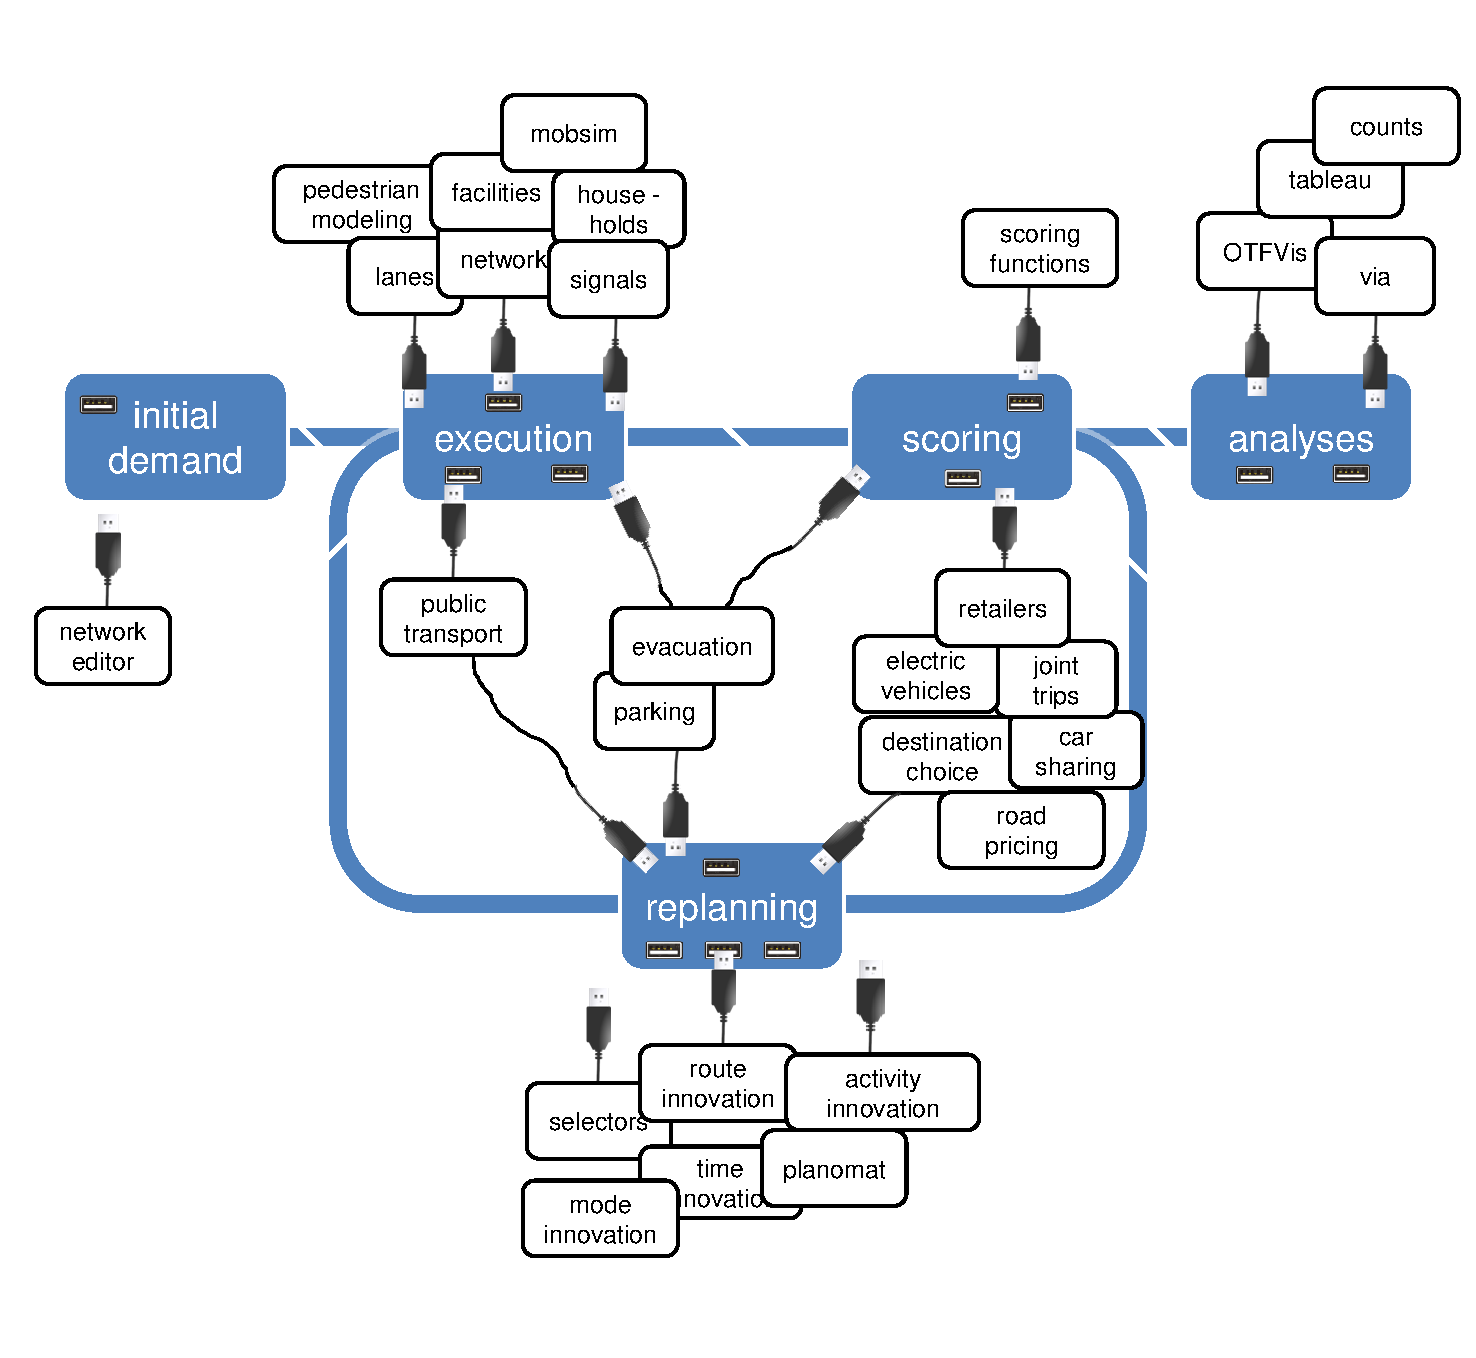
\includegraphics[width=0.99\textwidth, angle=0]{extending/figures/modules.pdf}}%
{}
%
The description of the modules in this and the following chapters is based on the categorization shown in Table~\ref{tab:modules}.
%
%\kai{TODO: macros for section names to re-use for table entries}
%\ah{Mache das später. Denke die jetzige Korrektur hält eine Weile}

\begin{center}
\begin{longtable}{|l|l|}
\caption{MATSim modules}
\label{tab:modules} 
%\hline
%\textbf{Module} & \textbf{Described in} \\
%\hline
\endfirsthead
\multicolumn{2}{c}%
{\tablename\ \thetable\ -- \textit{Continued from previous page}} \\
\hline
%\textbf{Module} & \textbf{Described in} \\
%\hline
\endhead
\hline \multicolumn{2}{r}{\textit{Continued on next page}} \\
\endfoot
\hline
\endlastfoot
	\hline
	\textbf{MATSim Data Containers} & Section~\ref{sec:matsim-containers} \\
	\hline
	Scenario &  Section~\ref{sec:scenario} \\
	Network  & Section~\ref{sec:lgstartednetwork} and \ref{sec:network} \\
	Population &  Section~\ref{sec:lgstarted-population} and \ref{sec:population} \\
	Counts  & Section~\ref{sec:counts} \\
	Facilities & Section~\ref{sec:facilities} \\
	Households &  Section~\ref{sec:households} \\
	Vehicles &  Section~\ref{sec:vehicles} \\
	\hline
	\textbf{Global Modules and Global Aspects} & Section~\ref{sec:globalmodules} \\
	\hline
	Controler &  Section~\ref{sec:using-controler} and \ref{sec:controler} \\
	Global &  Section~\ref{sec:global} \\
	Parallel Computing &  Section~\ref{sec:parallelcomputing} \\
	\hline
	\textbf{Mobsims} & Section~\ref{sec:using-mobsims} and \ref{sec:mobsims} \\
	\hline
	QSim &  Section~\ref{sec:using-qsim} and \ref{sec:qsim} \\
	JDEQSim &  Section~\ref{sec:jdeqsim} \\
	\hline
	\textbf{Scoring} & Section~\ref{sec:scoring} \\
	\hline
	\textbf{Strategy Modules} & Section~\ref{sec:strategymodules} \\
	\hline
	Time Innovation & Section~\ref{sec:timechoice} \\
	Route Innovation & Section~\ref{sec:routechoice} \\
	Mode Innovation & Section~\ref{sec:modechoice} \\
	Selectors & Section~\ref{sec:selectors} \\
	Destination Innovation & Chapter~\ref{ch:destinationchoice} \\
	\hline
	\textbf{Observational Modules} & Section~\ref{sec:observational} \\
	\hline
	Travel Time Calculator & Section~\ref{sec:ttc} \\
	Link Stats & Section~\ref{sec:linkStats} \\
	\hline
	\textbf{Further Modules Possibly Running in a \gls{matsim} Run} & \\
	\hline
	Within-day Replanning & Chapter~\ref{ch:withinday} \\
	Public Transport & Chapter~\ref{ch:pt} \\
	Multi-Modal Simulation & Chapter~\ref{ch:multimodalsim} \\
	Freight Traffic & Chapter~\ref{ch:freight} \\
	Car Sharing & Chapter~\ref{ch:carsharing} \\
	Joint Trips and Social Networks & Chapter~\ref{ch:jointtrips} \\
	Dynamic Transport Systems & Chapter~\ref{ch:dts} \\
	Parking & Chapter~\ref{ch:parking} \\
	Electric Vehicles & Chapter~\ref{ch:elvehicles} \\
	Air Transport & Chapter~\ref{ch:air} \\
	Roadpricing & Chapter~\ref{ch:roadpricing} \\
	Emissions & Chapter~\ref{ch:emissions} \\
	Accessibility & Chapter~\ref{ch:accessibility} \\
	Evacuation & Chapter~\ref{ch:evacuation}  \\
	Signals and Lanes & Chapter~\ref{ch:signalslanes} \\
	PSim & Chapter~\ref{ch:psim} \\
	\hline
	\textbf{Standalone Tools} & \\ % Out-Of-The-Loop Tools
	\hline
	Senozon via Visualizer & Chapter~\ref{ch:via} \\
	OTFVis Visualizer & Chapter~\ref{ch:otfvis} \\
	Cadyts & Chapter~\ref{ch:cadyts} \\
	\gls{matsim} For UrbanSim & Chapter~\ref{ch:matsim4urbansim} \\	
	Network Editors &  Chapter~\ref{ch:networkeditor} \\
	Interactive Analysis and Decision Support & Chapter~\ref{ch:businessanalytics} \\
\end{longtable}
\end{center}

% ##################################################################################################################
\section{MATSim Data Containers}
\label{sec:matsim-containers}
%% \subsection{Supply-Side Data Containers}
%% \label{sec:supplysidemodules}
% ======================================================
\subsection{Scenario}
\label{sec:scenario}

\begin{compactitem}
\item Invoking the module: (1) if you use Controler, scenario is always there. (2) otherwise, it needs to be generated explicitly in java.  \kai{chk}
\kai{Wir sind uns nicht im klaren darüber, was diese switches genau bedeuten, siehe \url{https://matsim.atlassian.net/browse/MATSIM-320}.  $\to$ weglassen.}

\item Configuration: There is a \lstinline|scenario| config file section, but we don't know what it means. \kai{chk}
%% \ah{Hier haben wir doch eine kleine Inkonsistenz zwischen Container und Configuration Section, oder?}

\item Configuration: \lstinline|scenario| config file section \ah{Hier haben wir doch eine kleine Inkonsistenz zwischen Container und Configuration Section. Config section definiert lanes, signals, households, vehicles, transit. Scenario hat aber z.B. facilities und population drin. Man sollte diese config section evtl. umbenennen in sowas wie optional\_scenario\_elements oder ähnlich. \url{https://matsim.atlassian.net/browse/MATSIM-320}}

\item Code: \lstinline|org.matsim.core.scenario|
\end{compactitem}

The \lstinline|scenario| module is
%, on the one hand, 
a container containing the main components of a scenario such as the \lstinline|config|, the \lstinline|network|, the \lstinline|population|, the \lstinline|facilities|, the \lstinline|transitSchedule|, \lstinline|households| and \lstinline|vehicles|.

%% The config file section is, on the other hand, used in a slightly different manner. It defines the usage of lanes, signal systems, road pricing, agent knowledges, vehicles, households and public transport. Still a respective config file section is required for every additional functionality. \kai{Ist das genau so?  Ich habe da ehrlich gesagt das genaue Design nie verstanden.  Oft für ein Eintrag in der scenario config group nur dafür, dass die Daten gelesen werden, und sonst passiert gar nichts.  Hm ...  Geradeziehen???}

% ===================================================================================
\subsection{Network}
\label{sec:network}
It is possible to make network attributes time-dependent, as observed in reality in case of accidents or adaptive traffic control, with varying speed limits or driving directions of lanes on multi-lane roads with heavily unbalanced load over the course of a day. Attributes that can be adapted are free speed, number of lanes and flow capacity.

The adaptation can be specified by adding following two lines to the \lstinline|network| configuration file section:
\begin{lstlisting}
<param name="timeVariantNetwork" value="true" />
<param name="inputChangeEventsFile" value="path_to_change_events_file" />
\end{lstlisting}
%
An example snippet setting the free speed of three network links to zero approximately looks as follows:
%
%% <?xml version="1.0" encoding="UTF-8"?>
%% 	<networkChangeEvents xmlns="http://www.matsim.org/files/dtd"
%% 	xmlns:xsi="http://www.w3.org/2001/XMLSchema-instance"
%% 	xsi:schemaLocation="http://www.matsim.org/files/dtd
%% 	http://www.matsim.org/files/dtd/networkChangeEvents.xsd">}
\begin{lstlisting}
  <networkChangeEvent startTime="03:06:00">
    <link refId="12487"/>
    <link refId="12489"/>
    <link refId="12491"/>
    <freespeed type="absolute" value="0.0"/>
  </networkChangeEvent>

\end{lstlisting}
%% </networkChangeEvents>
%
\kai{add reference to real file}
\ah{no suitable one found :(}

Alternatively, network change events can be directly added to the code using the method \lstinline|createNetworkChangeEvent| in class \lstinline|NetworkFactoryImpl|. An example can be found under \lstinline|org.matsim.integration.timevariantnetworks.QSimIntegrationTest| class. \ah{unfortunately no javadoc}
%
%\begin{lstlisting}
%networkChangeEvent =
	%network.getFactory().createNetworkChangeEvent(...);
%networkChangeEvent.setFlowCapacityChange(new ChangeValue(...));
%networkChangeEvent.setFreespeedChange(new ChangeValue(...));
%networkChangeEvent0.setLanesChange(new ChangeValue(...));
%network.addNetworkChangeEvent(networkChangeEvent);
%\end{lstlisting}
%
%\kai{lieber ein Verweis auf ein code snippet?  U.a. muss man auf NetworkImpl casten, was wir gerne irgendwann loswerden wollen und daher nicht im Buch haben wollen.}

% ===================================================================================
\subsection{Population}
\label{sec:population}
\begin{compactitem}
\item Invoking the module: By adding the respective configuration file section, the module is invoked automatically.
\item Configuration: \lstinline|plans| config file section. 
\item Code: \lstinline|org.matsim.core.population|
\end{compactitem}

The population module manages transport demand, i.e.,\,the population and the agents' plans.

\ah{das einzig relevante hier:} Optionally the path to a person attributes file in \lstinline|ObjectAttributes| format can be specified. 

% ===================================================================================
\subsection{Counts}
\label{sec:counts}
\begin{compactitem}
\item Invoking the module: By adding the respective configuration file section, the module is invoked automatically.
\item Configuration: \lstinline|counts| file section
\item Code: \lstinline|org.matsim.counts|
\end{compactitem}

\gls{matsim} offers the possibility to perform link volume comparisons between simulated and counted value for both motorized individual traffic \citep{Horni_unpub_IVT_2007}  and public transport. The later are described in Chapter \ref{ch:pt}. The count package offers analyses for the average working day with hourly resolution. A google maps based visualization is available, showing each station with a its load curve in a pop-up window at the geographic location.

As shown by \citet[][]{BalmerEtAl_ResRep_bdktzrh_2009}, for the Zürich scenario link volume comparisons have been successfully performed with data based on city level, cantonal level and national level \citep[][]{ASTRA_Webpage_2006}, where an average working day (Monday to Thursday, excluding public holidays) was built. Usually it is helpful to exclude a substantial part of the outer range of the modeled study region to prevent boundary effects.

\ah{merge if required:}
\begin{compactitem}
\item \lstinline|counts.xml| containing hourly volumes from real-world counting stations.
\end{compactitem}

\gls{matsim} provides funtionality to compare traffic volumes from your simulation to real world values. The Counts infrastructure allows to compare the traffic volumes on links on an hourly basis. The following listing shows an example of a \lstinline|counts.xml| input file required to do traffic count comparisons. 

\begin{xml}
<?xml version="1.0" encoding="UTF-8"?> 
<counts xmlns:xsi="http://www.w3.org/2001/XMLSchema-instance" 
        xsi:noNamespaceSchemaLocation="http://matsim.org/files/dtd/counts_v1.xsd" 
        name="test" desc="test counting stations" year="2014"> 
   <count loc_id="2" cs_id="005"> 
      <volume h="1" val="10.0"></volume> 
      <volume h="2" val="1.0"></volume> 
      <volume h="3" val="2.0"></volume> 
      <volume h="4" val="3.0"></volume> 
      <volume h="5" val="4.0"></volume> 
      <volume h="6" val="5.0"></volume> 
      <volume h="7" val="6.0"></volume> 
      <volume h="8" val="7.0"></volume> 
      <volume h="9" val="8.0"></volume> 
      <volume h="10" val="9.0"></volume> 
      <volume h="11" val="10.0"></volume> 
      <volume h="12" val="11.0"></volume> 
      <volume h="13" val="12.0"></volume> 
      <volume h="14" val="13.0"></volume> 
      <volume h="15" val="14.0"></volume> 
      <volume h="16" val="15.0"></volume> 
      <volume h="17" val="16.0"></volume> 
      <volume h="18" val="17.0"></volume> 
      <volume h="19" val="18.0"></volume> 
      <volume h="20" val="19.0"></volume> 
      <volume h="21" val="20.0"></volume> 
      <volume h="22" val="21.0"></volume> 
      <volume h="23" val="22.0"></volume> 
      <volume h="24" val="23.0"></volume> 
   </count> 
</counts>
\end{xml}
For a working example, check the \lstinline{examples/equil} directory in the \gls{matsim} directory tree (cf.\ Section~\ref{sec:settingUpMatsim}).

It starts with a header containing general descriptive information about the counts, including a year to describe how current the data is. Next, for each link having real world counts data, the hourly volumes can be specified. The network-link is referenced by the \lstinline|loc_id| attribute, in the example, it is link 2. The attribute \lstinline|cs_id| (counting station identifier) can be used to store an arbitrary description of the counting station. Most often it is used to note the original real word counting station to simplify future data comparison. The hourly volumes, specified by the hour of the day and its value, are optional: That is, not for every hour a value must be given. If for a counting station data is only available for certain hours of the day (e.g.,\,only during peak hours) it is possible to omit the other hours from the \gls{xml} listing.  Note that the first hour of the day, from 0:00 to 1:00, is numbered as ``1'', and \emph{not} by ``0'' as is often done in computer science.


% ===================================================================================
% -----------------------------------------------------------------------
\subsection{\lstinline|facilities.xml|}
\label{sec:facilitiescontainer}
In the facilities file location attributes can be specified. Importantly, open times and capacities can be added here. Facilities are not a mandatory element of core \gls{matsim}. Some \glspl{module}, such as the destination innovation module (Section~\ref{ch:destinationchoice}), use it, however.

%An example listing is as follows.
A facilities file approximately looks as follows:
%% <?xml version="1.0" encoding="UTF-8"?>
%% <!DOCTYPE facilities SYSTEM "http://www.matsim.org/files/dtd/facilities_v1.dtd">
\begin{xml}
...
<facilities name="test facilities for triangle network">
	<facility id="1" x="60.0" y="110.0">
		<activity type="home" />
	</facility>
	<facility id="10" x="110.0" y="270.0">
		<activity type="education" />
	</facility>
</facilities>
\end{xml}
A working example facilities file can be found in the \gls{matsim} directory tree in the \lstinline{examples/siouxfalls-2014} directory.

\subsection{Facilities}
\label{sec:facilities}
\begin{compactitem}
\item Invoking the module: By adding the respective configuration file section, the module is invoked automatically. Please make sure, that added modules can manage facilities.
\item Configuration: \lstinline|facilities| configuration file section
\item Code: \lstinline|org.matsim.core.facilities|
\end{compactitem}

Facilities are a non-mandatory element of \gls{matsim} scenarios. They identify activity locations and can hold opening hour and capacity information. facilities are mostly used in the \gls{matsim} Zürich group, in particular in the Zürich scenario, where facilities are derived from the Federal Enterprise Census 2001 \citep[][]{SwissEnterpriseCensus_manual_2001} providing hectare level information and using NOGA-classification. Detailed technical description of facilities generation is given by \citet[][]{Meister_TechRep_IVT_2008, Meister_unpub_IVT_2007}.

\ah{merge the following, if needed:}
\ah{If \gls{matsim} \glspl{facility} are used, the agents perform their activities in a specific \gls{facility} attached to a network link.
%
Generierung von Facilities muss/kann dann in Part II auch noch untergebracht werden: 

Clearly, many modules require further information about the infrastructure, in particular about the activity locations' open times. For the Swiss scenario the facilities are derived from a business census \citep[][]{SwissEnterpriseCensus_manual_2001}. Comparable data is available in most countries from official sources, such as censuses, and commercial sources, such as navigation network providers, yellow pages publishers or business directories, and last but not least google and \gls{osm} \citep[][]{OpenStreetMap_Webpage_2015}.
}

% ===================================================================================

% ##################################################################################################################
%% \subsection{Demand-Side Data Containers}
%% \label{sec:dsm}

% ===================================================================================
\subsection{Households}
\label{sec:households}
\begin{compactitem}
\item Invoking the module: Enable househlds in the \lstinline|scenario| section of the configuration file and provide the paths to a households file and another file containing the households' attributes in the configuration file section \lstinline|households|.
\item Configuration: \lstinline|households| config file section
\item Code: \lstinline|org.matsim.households|
\end{compactitem}

Similar to the vehicles module, the household module is not used by default in \gls{matsim}.

% ===================================================================================
%% \subsection{Data containers belonging both to demand and to supply}
\subsection{Vehicles}
\label{sec:vehicles}

%% A private household's decision to buy a vehicle in order to satisfy one's transport needs is a demand side decision.
%% %
%% However, if a public transit company decides to buy buses of a certain type, this is more a supply side decision (to supply potential passengers with a vehicle) than a demand side decision (the vehicle will have a demand for road space once it runs).

\begin{compactitem}
\item Invoking the module: Vehicles need to be enabled in the \lstinline|scenario| configuration file section.
\item Configuration: At the moment vehicles are only used for public transport (Chapter~\ref{ch:pt}), i.e.,\,motorized individual traffic vehicles are not used in \gls{matsim} nowadays. Thus, the configuration file section specifying the input file is located in the \lstinline|transit| configuration file section, while the vehicles module does not have its own configuration file section. 
\ah{Klären, ob man diese kleine Inkonsistenz beheben möchte.}  
\kai{Ist das nicht schon erledigt?}
\ah{final String vehiclesFile = this.config.transit().getVehiclesFile();}
\kai{Arghh.}
\ah{\url{https://matsim.atlassian.net/browse/MATSIM-314}}
%
This might change one day when the parking module will start to use vehicles. \citet[][]{JaeggiEtAl_TRR_2012} might serve as an empirical base for the assignment of vehicles to agents or households.
\item Code: \lstinline|org.matsim.vehicles|
\end{compactitem}

The vehicles package provides a file reader and a factory to create vehicles.

% -----------------------------------------------------------------------
\subsubsection{\lstinline|transitVehicles.xml|}
\label{sec:inputdata:transitvehicles}

\kai{convert to normal vehicles?}

To simulate public transport in \gls{matsim}, two additional input files are necessary. One is \lstinline|transitVehicles.xml|, which describes the vehicles which serve the lines: are they big buses, small buses, trains or light rail vehicles, and describes how many passengers each vehicle can transport.

The description of public transport vehicles can be split into two parts: In a first part, vehicle types have to be described, specifying how many passengers such a vehicle can transport (Note that the term "vehicle" can refer to multiple vehicles in reality, e.g.,\,a train with several wagons should be specified as one long vehicle with a high number of seats). In the second part, actual vehicles have to be listed. Each vehicle has an identifier and is of a previously specified vehicle type. The following shows an example of a such a file, describing one vehicle type and two vehicles of that type. 

\begin{xml}
<?xml version="1.0" encoding="UTF-8"?> 
<vehicleDefinitions xmlns="http://www.matsim.org/files/dtd" 
       xmlns:xsi="http://www.w3.org/2001/XMLSchema-instance" 
       xsi:schemaLocation="http://www.matsim.org/files/dtd http://www.matsim.org/files/dtd/vehicleDefinitions_v1.0.xsd"> 
	<vehicleType id="1"> 
      <description>Small Train</description> 
      <capacity> 
         <seats persons="50"/> 
         <standingRoom persons="30"/> 
      </capacity> 
      <length meter="50.0"/> 
   </vehicleType> 
   <vehicle id="tr_1" type="1"/> 
   <vehicle id="tr_2" type="1"/> 
</vehicleDefinitions>
\end{xml}

% -----------------------------------------------------------------------
\subsubsection{\lstinline|transitSchedule.xml|}
\label{sec:inputdata:transitschedule}
The second file that is required to simulate public transport is \lstinline|transitSchedule.xml|, a rather complex file. It contains information about stop facilities (these can be bus stops, train stations or other stop locations) and transit services.

In the first part, the stop facilities need to be defined, giving each one a coordinate, an identifier and a reference to a link in the network. The stop can only be served by vehicles driving on that specified link. Optionally, it is possible to specify a name for the stop and if other vehicles are blocked when a transit vehicle is waiting at a stop. This last attribute is useful to model e.g.,\,the difference of bus stops, where one bus stop has a bay, while at another stop, the bus has to stop on the actual road.

After the stop facilities, the transit lines, their routes and schedules are described. This is a hierarchical data structure: Each line can have one or more routes, each route has a route profile, a network route and a list of departures. The following listing represents an example of a minimalistic but complete transit schedule.
%
\begin{xml}
<?xml version="1.0" encoding="UTF-8"?> 
<!DOCTYPE transitSchedule SYSTEM "http://www.matsim.org/files/dtd/transitSchedule_v1.dtd"> 
<transitSchedule> 
   <transitStops> 
      <stopFacility id="1" x="990.0"  y="0.0"   name="Adorf" 
           linkRefId="1" isBlocking="false"/> 
      <stopFacility id="2" x="1100.0" y="980.0" name="Beweiler" 
           linkRefId="2" isBlocking="true"/> 
      <stopFacility id="3" x="0.0"    y="10.0"  name="Cestadt" 
           linkRefId="3" isBlocking="false"/> 
   </transitStops> 
   <transitLine id="Blue Line"> 
      <transitRoute id="1"> 
         <description>Just a comment.</description> 
         <transportMode>bus</transportMode> 
         <routeProfile> 
            <stop refId="1" departureOffset="00:00:00"/> 
            <stop refId="2" arrivalOffset="00:02:30" departureOffset="00:03:00" 
                                                     awaitDeparture="true"/> 
            <stop refId="3" arrivalOffset="00:05:00" awaitDeparture="true"/> 
         </routeProfile> 
         <route> 
            <link refId="1"/> 
            <link refId="2"/> 
            <link refId="3"/> 
         </route> 
         <departures> 
            <departure id="1" departureTime="07:00:00" vehicleRefId="12"/> 
            <departure id="2" departureTime="07:05:00" vehicleRefId="23"/> 
            <departure id="3" departureTime="07:10:00" vehicleRefId="34"/> 
         </departures> 
      </transitRoute> 
   </transitLine> 
</transitSchedule>
\end{xml}

Each transit line must have a unique id. Each transit route has an id which must be unique within that one line, so the same route id can be used with different lines. The \lstinline|transportMode| describes on which links in the network the line runs (Actually, this is currently not yet enforced. It would be possible to let a bus run on train links in the simulation. It might be enforced in the future).

The \lstinline|routeProfile| describes the stops this route serves, while route itself describes the series of links in the network the transit vehicle's driver has to drive along (thus often referred to as network route. Note that the complete route, i.e.,\,all links the vehicle drives along, must be listed in the route, and not only the ones where stops are located. All the specified stops should occur along this route in the specified order. The time offsets given for each stop in the \lstinline|routeProfile| describe the relative time offset to an actual departure time. If a bus is to depart at 7\,am, and stop 2 has a \lstinline|departureOffset| 3\,minutes, this must be read that the bus is expected to depart at 7:03\,am at the specific stop. All stops in the route profile must have a departure offset defined, except the last one. All stops, except the first one, can optionally have an arrival offset defined. This is mostly useful for large trains that stop for several minutes at a station to help the routing algorithm to find connecting services at the correct time, namely the expected arrival time of the train.

As last part of the description of a transit route, the list of departures should be given. Each departure has an id, which must be unique within the route, and gives the departure time at the first stop of the specified route profile. In addition, the departure specifies with which vehicle the service should be run. This vehicle must be defined in the aforementioned list of transit vehicles. 

Because of its complexity, transit schedules often contain little mistakes that will return in an error when the simulation runs. Typical examples include that the network route is missing a link, or that the network route does not pass at all the defined stops in the right order. To make sure a schedule does not have any such issues before the simulation is started, a special validation routine is available:

\begin{lstlisting}
java -Xmx512m -cp /path/to/matsim.jar  
      org.matsim.pt.utils.TransitScheduleValidator  
      /path/to/transitSchedule.xml /path/to/network.xml
\end{lstlisting}

If run, this validator will print out a list of errors or warnings, if any are found, or show a message that the schedule appears to be valid.

\ah{merge if required:}
\ah{In the beginning of \gls{matsim} only car mode could be simulated. With the addition of the public transport \gls{module} (Chapter~\ref{ch:pt}), with the help of two further input files public transport can just as well be simulated:
\begin{compactitem}
\item \lstinline|transitVehicles.xml| providing the description of the vehicles used for public transport services. \kai{vehicles.xml?  (without ``transit''?)} \kai{Andreas, fyi: I think we are leaning towards having separate containers vehicles.xml and transitVehicles.xml.  Not yet implemented.}
\item \lstinline|transitSchedule.xml| containing information about transit stop locations and transit services,
\end{compactitem}
%
} 

%##################################################################################################################
\section{Global Modules and Global Aspects}
\label{sec:globalmodules}
% ===================================================================================
\subsection{Controler}
\label{sec:controler}
The module, can be extended by \lstinline|Events| and \lstinline|Listeners| as detailed in Chapter~\ref{ch:extensionpoints}. 
%% Classes implementing one or more \lstinline|Listener Interfaces| and can be registered with the Controler with \lstinline|addControlerListener()|. The controler fires \lstinline|Controler Events| at specific points during the run to the registered \lstinline|Listeners|, which can then execute their own code.
%
%Das ist nur ein Ausschnitt von dem, was der Controler kann.  Da es im entsprechenden Kap. ja beschrieben wird, brauchen wir das hier m.E. nicht nochmal. kai, dec'14

%% \textcolor{gray}{\st{Another possibility to customize the controler is by inheritence from the class} \lstinline|org.matsim.core.controler|.}  \kai{Please do not do or advertise this any more.}

% ##################################################################################################################
\section{\protect\glspl{mobsim}}
\label{sec:mobsims}
% ===================================================================================
\subsection{\protect\gls{qsim}}
\label{sec:qsim}
The simulation is able to handle time-variant networks, within-day replanning \citep[][]{Dobler_TechRep_IVT_2009}, multi-modal scenarios (Section~\ref{sec:multimodalsim_qsim}) and in an experimental manner also traffic lights \citep[][]{Neumann_MastersThesis_2008}).

% --------------------------------------
\subsubsection{Multi-Modal Simulation With QSim}
\label{sec:multimodalsim_qsim}
\gls{qsim} can simulate \gls{multimodal} traffic. Congested modes, i.e.,\,modes simulated not only teleported, are specified by the parameter \lstinline|mainMode|. Technically, these are the modes that the departure handler of the \lstinline|netsimengine| handles 
\footnote{Effective cell size, effective lane width, flow capacity factor, and storage capacity factor need to be set with diligence.}. 
Theoretically also pedestrians can be included, however, only vehicular modes actually make sense, i.e.,\,car, bike, and public transport, in particular buses. 
\ah{Is that true with pt? Do we actually have all the vehicular traffic interactions in \gls{qsim}?}. 
Assigning vehicles of a specific type to agents is done with in the vehicles input file \lstinline|<param name="vehiclesFile" value="..." />|. 
\ah{is that the only place necessary?}. 
Further configuration necessary to include public transport is detailed in Chapter~\ref{ch:pt}.

To model multi-modal interactions, a fully multi-modal network, i.e.,\,a network that has links being shared by different modes must be provided. 
As shown in Section~\ref{sec:lgstartednetwork}, specification of link modes is done with the network attribute \lstinline|modes|.
Furthermore, the router needs to be informed about the network modes by the \lstinline|planscalcroute| parameter \lstinline|<param name="networkModes" value="car,ride" />|.
\ah{is this a double configuration, qsim and planscalcroute? can we merge them?}

The mode interactions can be further specified by \gls{qsim} parameter \lstinline|linkDynamics|. 
This parameter is also productive for car mode only, but it is particularly important for multi-modal scenarios. 
Dynamics either follow strict \gls{fifo} or include passing, i.e.,\,\lstinline$<param name="linkDynamics" value="FIFO|PassingQ" />$. 
Passing is all-or-none, i.e.,\,either every vehicle type can pass every other type or none can pass none. 
However, in reality, there usually is something between \gls{fifo} and free passing, e.g.,\,a bus might not be able to pass a car, although being faster, whereas bikes might always be able to slip by cars. Such more fine-grained rules about passing do not yet exist at the time of writing this book. 

Simulation experiments for \gls{qsim}'s relatively new multi-modal feature have been performed for the Patna scenario as reported in Section~\ref{sec:patna}.

An earlier multi-modal approach targeted at overcoming the teleportation estimates of non-motorized modes, particularly focused on pedestrians, is presented in Chapter~\ref{ch:multimodalsim}.

\ah{Please check all of that. Thanks.}

% ##################################################################################################################
% Local Variables:
% mode: latex
% mode: reftex
% mode: visual-line
% TeX-master: "../../main"
% comment-padding: 1
% fill-column: 9999
% End: 
